% Тип документа
\documentclass[a4paper,14pt]{extarticle}

% Шрифты, кодировки, символьные таблицы, переносы
\usepackage{cmap}
\usepackage[T2A]{fontenc}
\usepackage[utf8x]{inputenc}
\usepackage[russian]{babel}
\usepackage[table]{xcolor}
% Это пакет -- хитрый пакет, он нужен но не нужен
\usepackage[mode=buildnew]{standalone}

\usepackage
	{
		% Дополнения Американского математического общества (AMS)
		amssymb,
		amsfonts,
		amsmath,
		amsthm,
		physics,
		% misccorr,
		% 
		% Графики и рисунки
		wrapfig,
		graphicx,
		subcaption,
		float,
		tikz,
		tikz-3dplot,
		caption,
		csvsimple,
		color,
		booktabs,
		pgfplots,
		pgfplotstable,
		geometry,
		% 
		% Таблицы, списки
		array,
		makecell,
		multirow,
		indentfirst,
		%
		% Интегралы и прочие обозначения
		ulem,
		esint,
		esdiff,
		% 
		% Колонтитулы
		fancyhdr,
	}  

\usepackage{xcolor}
\usepackage{hyperref}

 % Цвета для гиперссылок
\definecolor{linkcolor}{HTML}{000000} % цвет ссылок
\definecolor{urlcolor}{HTML}{799B03} % цвет гиперссылок
 
\hypersetup{pdfstartview=FitH,  linkcolor=linkcolor,urlcolor=urlcolor, colorlinks=true}
% Обводка текста в TikZ
\usepackage[outline]{contour}

% Увеличенный межстрочный интервал, французские пробелы
\linespread{1.1} 
\frenchspacing 

 
\usetikzlibrary
	{
		decorations.pathreplacing,
		decorations.pathmorphing,
		patterns,
		calc,
		scopes,
		arrows,
		fadings,
		through,
		shapes.misc,
		arrows.meta,
		3d,
		quotes,
		angles,
		babel
	}

\usepgfplotslibrary{units}

% const прямым шрифтом
\newcommand\ct[1]{\text{\rmfamily\upshape #1}}
\newcommand*{\const}{\ct{const}}
\renewcommand*{\epsilon}{\varepsilon}

\usepackage[europeanresistors,americaninductors]{circuitikz}

% Style to select only points from #1 to #2 (inclusive)
\pgfplotsset{select/.style 2 args={
    x filter/.code={
        \ifnum\coordindex<#1\def\pgfmathresult{}\fi
        \ifnum\coordindex>#2\def\pgfmathresult{}\fi
    }
}}

\usepackage{array}
\usepackage{pstool}

%%%%%%%%%%%%%%%%%%%%%%%%%%%%%%%%%%%%%%%%%%%%%%%%%
\makeatletter
\newif\if@gather@prefix 
\preto\place@tag@gather{% 
  \if@gather@prefix\iftagsleft@ 
    \kern-\gdisplaywidth@ 
    \rlap{\gather@prefix}% 
    \kern\gdisplaywidth@ 
  \fi\fi 
} 
\appto\place@tag@gather{% 
  \if@gather@prefix\iftagsleft@\else 
    \kern-\displaywidth 
    \rlap{\gather@prefix}% 
    \kern\displaywidth 
  \fi\fi 
  \global\@gather@prefixfalse 
} 
\preto\place@tag{% 
  \if@gather@prefix\iftagsleft@ 
    \kern-\gdisplaywidth@ 
    \rlap{\gather@prefix}% 
    \kern\displaywidth@ 
  \fi\fi 
} 
\appto\place@tag{% 
  \if@gather@prefix\iftagsleft@\else 
    \kern-\displaywidth 
    \rlap{\gather@prefix}% 
    \kern\displaywidth 
  \fi\fi 
  \global\@gather@prefixfalse 
} 
\newcommand*{\beforetext}[1]{% 
  \ifmeasuring@\else
  \gdef\gather@prefix{#1}% 
  \global\@gather@prefixtrue 
  \fi
} 
\makeatother
%%%%%%%%%%%%%%%%%%%%%%%%%%%%%%%%%%%%%%%%%%%%%%%%%

\geometry		
	{
		left			=	2cm,
		right 			=	2cm,
		top 			=	3cm,
		bottom 			=	3cm,
		bindingoffset	=	0cm
	}

%%%%%%%%%%%%%%%%%%%%%%%%%%%%%%%%%%%%%%%%%%%%%%%%%%%%%%%%%%%%%%%%%%%%%%%%%%%%%%%

	%применим колонтитул к стилю страницы
\pagestyle{fancy} 
	%очистим "шапку" страницы
\fancyhead{} 
	%слева сверху на четных и справа на нечетных
\fancyhead[R]{\labauthors} 
	%справа сверху на четных и слева на нечетных
\fancyhead[L]{Отчёт по лабораторной работе №\labnumber} 
	%очистим "подвал" страницы
\fancyfoot{} 
	% номер страницы в нижнем колинтуле в центре
\fancyfoot[C]{\thepage} 

%%%%%%%%%%%%%%%%%%%%%%%%%%%%%%%%%%%%%%%%%%%%%%%%%%%%%%%%%%%%%%%%%%%%%%%%%%%%%%%

\renewcommand{\contentsname}{Оглавление}

\usepackage{tocloft}
% \renewcommand{\cftpartleader}{\cftdotfill{\cftdotsep}} % for parts
% \renewcommand{\cftsectiondotsep}{\cftdotsep}% Chapters should use dots in ToC
\renewcommand{\cftsecleader}{\cftdotfill{\cftdotsep}}
%\renewcommand{\cftsecleader}{\cftdotfill{\cftdotsep}} % for sections, if you really want! (It is default in report and book class (So you may not need it).
% ---------
% \newcommand{\cftchapaftersnum}{.}%
% \usepackage{titlesec}
% \titlelabel{\thetitle.\quad}
\usepackage{secdot}
\sectiondot{subsection}
\newcommand{\rot}{\operatorname{rot}}
\newcommand{\vH}{\textbf{H}}
\newcommand{\vE}{\textbf{E}}
\newcommand{\vB}{\textbf{B}}
\newcommand{\vD}{\textbf{D}}
\newcommand{\vr}{\textbf{r}}
\newcommand{\vj}{\textbf{j}}
\newcommand{\vk}{\textbf{k}}
\newcommand{\vx}{\textbf{x}}
\newcommand{\vy}{\textbf{y}}
\newcommand{\vz}{\textbf{z}}
\begin{document}

\def\labauthors{Карусевич А.А., Шиков А.П.}
\def\labgroup{440}
\def\labnumber{1}
\def\labtheme{Волноводные ферритовые устройства СВЧ диапазона}
\begin{titlepage}

\begin{center}

{\small\textsc{Нижегородский государственный университет имени Н.\,И. Лобачевского}}
\vskip 1pt \hrule \vskip 3pt
{\small\textsc{Радиофизический факультет. Кафедра Электродинамики.}}

\vfill

{\Large Отчет по лабораторной работе №\labnumber\vskip 12pt\bfseries \labtheme}
	
\end{center}

\vfill
	
\begin{flushright}
	{Выполнили студенты \labgroup\ группы\\ \labauthors}%\vskip 12pt Принял:\\ Менсов С.\,Н.}
\end{flushright}
	
\vfill
	
\begin{center}
	Нижний Новгород, \the\year
\end{center}

\end{titlepage}



\newpage

{\bfseries Цель работы:} 
Изучение электродинамических систем, содержащих гиротропные элементы - ферриты.

\section{Теоритическая часть}
\subsection{Введение}
Известно, что в линейных анизотропных средах с симметричными тензорами диэлектрической и магнитной проницаемости
$\epsilon_{ij} = \epsilon_{ji},\mu_{ij} = \mu_{ji}$ (а также в обычных изотропных средах) имеет место теорема взаимности. Эта теорема оказывается несправедливой в средах
с несимметричными тензорами проницаемостей, в частности, в так называемых гиротропных средах, к которым принадлежат
плазма и ферриты, находящиеся во внешнем постоянном магнитном ноле.

Используя невзаимные свойства гиротропных сред, можно создавать устройства, канализирующие электромагнитные волны в
одном направлении и почти не пропускающие в противоположном направлении. Этим объясняется широкое применение ферритов в
волноводных устройствах сверхвысокочастотного (СВЧ) диапазона. К настоящему времени разработано большое количество
устройств с ферритовыми элементами, имеющих различные конструктивные исполнения и электродинамические характеристики.

\subsection{Анизотропные и гиротропные среды}

Анизотропными средами называются среды, локальные макроскопические свойства которых различны в различных направлениях. Поликристаллические вещества становятся анизотропными
под воздействием давления, статических электрических и магнитных полей. Наряду с анизотропными существуют среды,
локальные макроскопические свойства которых неинвариантны относительно зеркальных отражений, т.е. изменяются при
некоторых зеркальных отражениях. Такие среды называются естественноактивными (пли гиротропными). Примерами таких сред
могут служить кристаллы без центра симметрии или среды, состоящие из частиц, не обладающих центром симметрии. Некоторые
среды приобретают гиротропные свойства при наложении внешнего магнитного поля. Такие среды принято называть
магнитоактивными. Типичными примерами магнитоактивных сред являются плазма и ферриты, находящиеся во внешнем постоянном
магнитном поле.

\textit{Ферриты}, представляют собой химические соединения оксида железа с оксидами других, так называемых характеризующих
металлов (никеля, кобальта, магния, марганца, кадмия и т. д.). Особенностью этих материалов является сочетание
гиротропных свойств с низкой электропроводностью, благодаря чему электромагнитные волны при определенных условиях могут
распространяться в ферритах с достаточно малым затуханием.

Магнитные свойства ферритов определяются наличием в их кристаллической решетке атомов или ионов, обладающих отличным от
нуля магнитным моментом. В отсутствие внешнего магнитного поля магнитные моменты ориентированы хаотически, и в целом
феррит изотропен. В достаточно сильном постоянном магнитном поле $\vH_0$ магнитные моменты всех атомов за время
$\tau_0 \simeq (10^{-9} - 10^{-7})$ с (время релаксации) устанавливаются по направлению магнитного поля. В этом состоянии феррит обладает
значительной намагниченностью и становится анизотропной гиротропной средой по отношению к высокочастотному электромагнитному полю.

В линейном анизотропном магнетике каждая компонента вектора магнитной индукции $\vB$ представляет собой линейную функцию
трех компонент ноля $\vH$:
\begin{equation}
    \begin{aligned} 
        B_{x} &=\mu_{x x} H_{x}+\mu_{x y} H_{y}+\mu_{x z} H_{z} \\
        B_{y} &=\mu_{y x} H_{x}+\mu_{y y} H_{y}+\mu_{y z} H_{z} \\
        B_{z} &=\mu_{z x} H_{x}+\mu_{z y} H_{y}+\mu_{z z} H_{z}
    \end{aligned}
    \label{eq:1}
\end{equation}
Величины $\mu_{i j}(i,j=x,y,z)$, входящие в соотношения \eqref{eq:1}, являются компонентами тензора второго ранга, называемого
тензором магнитной проницаемости:
\begin{equation}
    \hat{\mu}=\left(\begin{array}
        {ccc}{\mu_{x x}} & {\mu_{x y}} & {\mu_{x z}} \\
        {\mu_{y x}} & {\mu_{y y}} & {\mu_{y z}} \\
        {\mu_{z x}} & {\mu_{z y}} & {\mu_{z z}}
    \end{array}\right)
    \label{eq:2}
\end{equation}


С учетом \eqref{eq:2} материальные уравнения \eqref{eq:1} можно записать в удобной матричной форме

\begin{equation}
    \textbf{B} = \hat{\mu}\textbf{H}
    \label{eq:3}
\end{equation}

При наличии в феррите электромагнитного поля, изменяющегося во времени но гармоническому закону и имеющего напряженность
$\vH(\vr)e^{i\omega t}$, малую но сравнению с постоянным магнитным полем $\textbf{H}_0 =
H_0\textbf{z}_0(|\vH|\ll H_0)$, тензор магнитной проницаемости $\hat{\mu}$ принимает вид

\begin{equation}
    \hat{\mu}=\left(\begin{array}
        {ccc}{\mu} & {i\mu_{a}} & {0} \\
        {-i\mu_{a}} & {\mu} & {0} \\
        {0} & {0} & {\mu_{||}}
    \end{array}\right)
    \label{eq:4}
\end{equation}

\begin{equation}
    \mu=1+\frac{4 \pi \chi \omega_{H}^{2}}{\omega_{H}^{2}-\omega^{2}}, 
    \quad \mu_{a}=\frac{4 \pi \chi \omega_{H} \omega}{\omega_{H}^{2}-\omega^{2}}, 
    \quad \mu_{ \|}=1
    \label{eq:5}
\end{equation}
Здесь $\omega$ - круговая частота, $\chi$ - статическая магнитная восприимчивость феррита, $\omega_H = \frac{e H_0}{m
c}$ - гирочастота электрона ($m$ и $e$ — масса и абсолютное значение заряда электрона соответственно, $c$ — скорость света в вакууме).


Обратим внимание на то, что тензор \eqref{eq:4} подчиняется соотношению $\mu_{ij} = \mu_{ji}^*$ т. е. является эрмитовым (знак «*» означает
операцию комплексного сопряжения). Данное свойство имеет место для сред при пренебрежении потерями.

В отсутствие статического магнитного поля $(\textbf{H}_0 = 0)$ недиагональные элементы тензора \eqref{eq:4} обращаются в пуль, диагональные
компоненты $\mu$ и $\mu_{||}$ принимают одинаковые значения ($\mu=\mu_{||}$), и феррит становится изотропным.

При стремлении частоты поля $\omega$ к гирочастоте $\omega_H$ компоненты $\mu$ и $\mu_a$ обращаются в бесконечность. Это явление называют
ферромагнитным резонансом. В действительности из-за диссипативных процессов элементы тензора $\mu$ и $\mu_a$ становятся весьма
большими, но не бесконечными. Потери в феррите в случае малой диссипации можно учесть феноменологически , заменив
частоту $\omega_H$ в выражениях \eqref{eq:5} па комплексную величину $\tilde{\omega}_H = \omega_H+ i \gamma \omega$, где
$\gamma$ — безразмерный параметр диссипации ($\gamma \ll 1$).

\begin{figure}[h!]
    \centering
    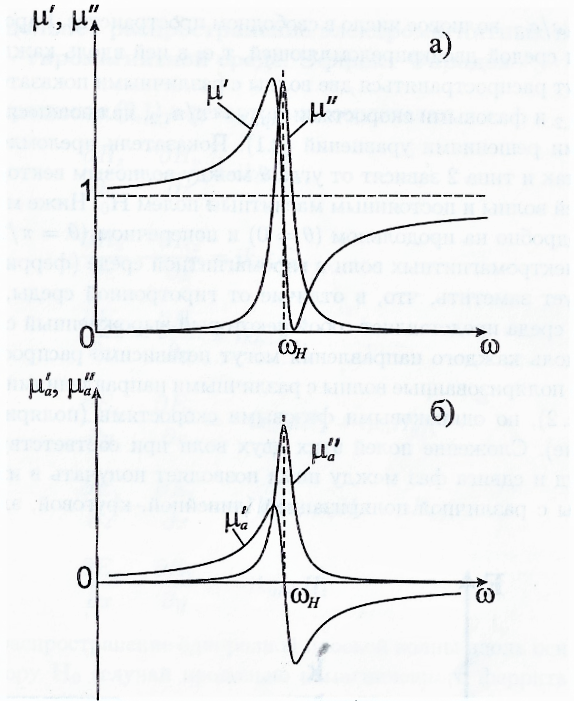
\includegraphics[width = 0.5\linewidth]{imgs/temp/001.png}
    \caption{Качественный вид зависимостей величин $\mu^{\prime}$, $\mu^{\prime \prime}(a)$ и 
    $\mu_{a}^{\prime}$, $\mu_{a}^{\prime \prime}$(b) от частоты $\omega$}
    \label{fig:1}
\end{figure}

Таким образом, при учете потерь величины $\mu$ и $\mu_{a}$ являются комплексными, т. е. $\mu=\mu^{\prime}-i \mu^{\prime \prime}, 
\mu_{a}=\mu_{a}^{\prime}-i \mu_{a}^{\prime \prime}$, а тензор $\hat{\mu}$ перестает быть эрмитовым ($\mu_{ij} \neq
\mu_{ji}^*$). Качественные зависимости действительных и мнимых частей этих величин от частоты
$\omega$ при фиксированном статическом поле $H_0$ показаны на рис. \ref{fig:1}. Из рис. \ref{fig:1} видно, что в случае $\omega=\omega_H$ и
величины $\mu^{\prime \prime}$ и $\mu_{a}^{\prime \prime}$ максимальны, что свидетельствует о резонансном поглощении
электромагнитного поля ферритом. Следует отметить, что в ограниченных ферритовых образцах внутреннее статическое
магнитное поле $\vH_0$ отличается от внешнего поля $\vH_{\text{ВН}}$, в которое
помещен образец. Поэтому частота ферромагнитного резонанса при заданном поле $\vH_{\text{ВН}}$ зависит от формы образца и его
ориентации относительно внешнего магнитного поля. Для определения внутреннего ноля в образце следует решить
соответствующую краевую задачу магнитостатики.

\subsection{Распространение электромагнитных волн в гиротропной среде}
Рассмотрим неограниченную гиротропную среду с тензором магнитной проницаемости \eqref{eq:4} и скалярной диэлектрической
проницаемостью $\epsilon$. Такую среду принято называть гиромагнитной. Уравнения Максвелла для комплексных амплитуд
$\vE(\vr)$, $\vH(\vr)$ в гиромагнитной среде без источников ($\vj^e = \vj^m=0$) имеют вид
\begin{equation}
    \rot \vE=-i k_{0} \hat{\mu} \vH, \quad \rot \vH=i k_{0} \epsilon \vE
    \label{eq:2:1}
\end{equation}
где $k_0 = \omega /c$ — волновое число в свободном пространстве. Гиротропная среда является средой двоякопреломляющей, т. е. в
ней вдоль каждого направления могут распространяться две волны с различными показателями преломления $n_{1,2}$ и фазовыми
скоростями $v_{\text{ф}1,2} = c/n_{1,2}$, являющиеся линейно независимыми решениями уравнений \eqref{eq:2:1}. Показатели преломления волн как
типа 1, так и типа 2 зависят от угла $\theta$ между волновым вектором $\vk$ соответствующей волны и постоянным магнитным полем $\vH_0$.

Следует заметить, что, в отличие от гиротропной среды, обычная изотропная среда представляет собой некоторый вырожденный
случай, так как в ней вдоль каждого направления могут независимо распространяться две линейно поляризованные волны с
различными направлениями векторов поля, но одинаковыми фазовыми скоростями (поляризационное вырождение).
Сложение полей этих двух волн при соответствующем выборе амплитуд и сдвига фаз между ними позволяет получать в
изотропной среде волны с различной поляризацией (линейной, круговой, эллиптической).
В анизотропных и гиротроппых средах поляризационное вырождение отсутствует, и каждой волне с определенным значением
показателя преломления соответствует фиксированная поляризация, отличающаяся в общем случае от линейной.

\subsubsection{Продольное распространение электромагнитных волн в гиромагнитной среде. Эффект Фарадея}
% Запишем уравнения \eqref{eq:2:1} в декартовых координатах:
% \begin{equation}
%     \begin{aligned}
%         &\frac{\partial H_{z}}{\partial y}-\frac{\partial H_{y}}{\partial z}=i k_{0} \epsilon E_{x},\\
%         &\frac{\partial H_{x}}{\partial z}-\frac{\partial H_{z}}{\partial x}=i k_{0} \epsilon E_{y},\\
%         &\frac{\partial H_{y}}{\partial x}-\frac{\partial H_{x}}{\partial y}=i k_{0} \varepsilon E_{z},\\
%         &\frac{\partial E_{z}}{\partial y}-\frac{\partial E_{y}}{\partial z}=-i k_{0}\left(\mu H_{x}+i \mu_{a} H_{y}\right),\\
%         &\frac{\partial E_{x}}{\partial z}-\frac{\partial E_{z}}{\partial x}=-i k_{0}\left(-i \mu_{a} H_{x}+\mu H_{y}\right),\\
%         &\frac{\partial E_{y}}{\partial x}-\frac{\partial E_{x}}{\partial y}=-i k_{0} \mu_{ \|} H_{z}
%     \end{aligned}
%     \label{eq:2:2}
% \end{equation}
% Рассмотрим распространение однородной плоской волны вдоль оси z, параллельной вектору $\vH_0$ (случай продольно
% намагниченного феррита). В этом случае уравнения \eqref{eq:2:2} принимают вид $\left(\vE(\vr), \vH(\vr) \propto e^{-i h
% z}\right)$
% \begin{equation}
%     \begin{array}
%     {cl}{h H_{y}=k_{0} \epsilon E_{x},} & {h E_{y}=-k_{0}\left(\mu H_{x}+i \mu_{a} H_{y}\right)}, \\
%     {h H_{x}=-k_{0} \epsilon E_{y},} & {h E_{x}=k_{0}\left(-i \mu_{a} H_{x}+\mu H_{y}\right)}, \\
%     {} & {E_{z}=H_{z}=0}
%     \end{array}
%     \label{eq:2:3}
% \end{equation}
% Из \eqref{eq:2:3} получаем
% \begin{equation}
% \begin{array}
%     {l}{i k_{0}^{2} \epsilon \mu_{a} E_{x}+\left(h^{2}-k_{0}^{2} \varepsilon \mu\right) E_{y}=0} \\
%      {\left(h^{2}-k_{0}^{2} \varepsilon \mu\right) E_{x}-i k_{0}^{2} \varepsilon \mu_{a} E_{y}=0}
%     \end{array}
%     \label{eq:2:4}
% \end{equation}
% Система линейных уравнений \eqref{eq:2:4} имеет нетривиальное решение, если ее определитель равен нулю:
% \begin{equation}
%     (h^2-k_0^2 \epsilon \mu)^2-k_0^4\epsilon^2\mu_a^2=0,
%     \label{eq:2:5}
% \end{equation}
% откуда следует
% \begin{equation}
%     h_{1,2}^{2}=k_{0}^{2} \varepsilon\left(\mu \pm \mu_{a}\right)
%     \label{eq:2:6}
% \end{equation}
В продольно намагниченном феррите могут распространяться две поперечные волны с различными постоянными
распространения, т.е. с различными фазовыми скоростями и затуханиями.

Для волны, бегущей в положительном направлении оси z с постоянной распространения $h_{1}=k_{0} n_{1}=k_{0} \sqrt{\epsilon\left(\mu+\mu_{a}\right)}$, из
уравнений \eqref{eq:2:3}-\eqref{eq:2:6} имеем соотношения
\begin{equation}
    E_{x}=i E_{y}, \quad H_{x}=i H_{y}, \quad \frac{E_{x}}{H_{y}}=-\frac{E_{y}}{H_{x}}=\sqrt{\frac{\mu+\mu_{a}}{\varepsilon}}
    \label{eq:2:7}
\end{equation}
а для волны с постоянной распространения $h_{2}=k_{0} n_{2}=k_{0} \sqrt{\varepsilon\left(\mu-\mu_{a}\right)}$ —
соотношения
\begin{equation}
    E_{x}=-i E_{y}, \quad H_{x}=-i H_{y}, \quad \frac{E_{x}}{H_{y}}=-\frac{E_{y}}{H_{x}}=\sqrt{\frac{\mu-\mu_{a}}{\varepsilon}}
    \label{eq:2:8}
\end{equation}
Полученные выражения показывают, что поля $\vE$ и $\vH$ обеих волн взаимно перпендикулярны и поляризованы по кругу с правым
направлением вращения векторов $\vE,\vH$ относительно направления постоянного магнитного поля $\vH_0$ у первой волны ($h_1$) и с
левым — у второй ($h_2$).

Из \eqref{eq:2:3}-\eqref{eq:2:7} следует, что для правополяризованной волны, распространяющейся в положительном направлении оси $z$, справедливы соотношения
\begin{equation}
    \begin{array}
    {ll}{\vE=E_{0}\left(\vx_{0}-i \vy_{0}\right) e^{-i h_{1} z},} & {\vH=\sqrt{\frac{\epsilon}{\mu_{1}}} E_{0}\left(i \vx_{0}+\vy_{0}\right) e^{-i h_{1} z}}, \\
    {h_{1}=k_{0} \sqrt{\varepsilon \mu_{1}}=\alpha_{1}-i \beta_{1},} & {v_{\text{ф} 1}=\omega / \alpha_{1}},\end{array}
    \label{eq:2:9}
\end{equation}

где $\mu_{1}=\mu+\mu_{a}=\mu_{1}^{\prime}-i \mu_{1}^{\prime \prime}$ - эквивалентная магнитная проницаемость (см. рис. \ref{fig:3}), $v_{\text{ф}1}$ — фазовая скорость волны.

Магнитная проницаемость $\mu_{1}$ при значениях $\omega_{H}$, близких к круговой частоте волны $\omega$ (то есть при
магнитном поле $\vH_0$, близком к резонансному значению $H_{\text{рез}} = \frac{mc\omega}{e}$ (см. рис. \ref{fig:3})) имеет
большую мнимую часть. Поэтому правополяризованная волна может испытывать значительное резонансное поглощение.

Для левополяризованной волны, распространяющейся в положительном направлении оси $z$, имеем
\begin{equation}
    \begin{array}
    {ll}{\vE=E_{0}\left(\vx_{0}+i \vy_{0}\right) e^{-i h_{2} z},} & {\vH=\sqrt{\frac{\epsilon}{\mu_{2}}} E_{0}\left(-i \vx_{0}+\vy_{0}\right) e^{-i h_{2} z}}, \\
    {h_{2}=k_{0} \sqrt{\varepsilon \mu_{2}}=\alpha_{2}-i \beta_{2},} & {v_{\text{ф} 2}=\omega / \alpha_{2}},\end{array}
    \label{eq:2:10}
\end{equation}
где $\mu_{2}=\mu+\mu_{a}=\mu_{2}^{\prime}-i \mu_{2}^{\prime \prime}$.
Эта волна, в отличие от правополяризованной, не испытывает резонансного поглощения (рис. \ref{fig:3}).
\begin{figure}[h!]
    \centering
    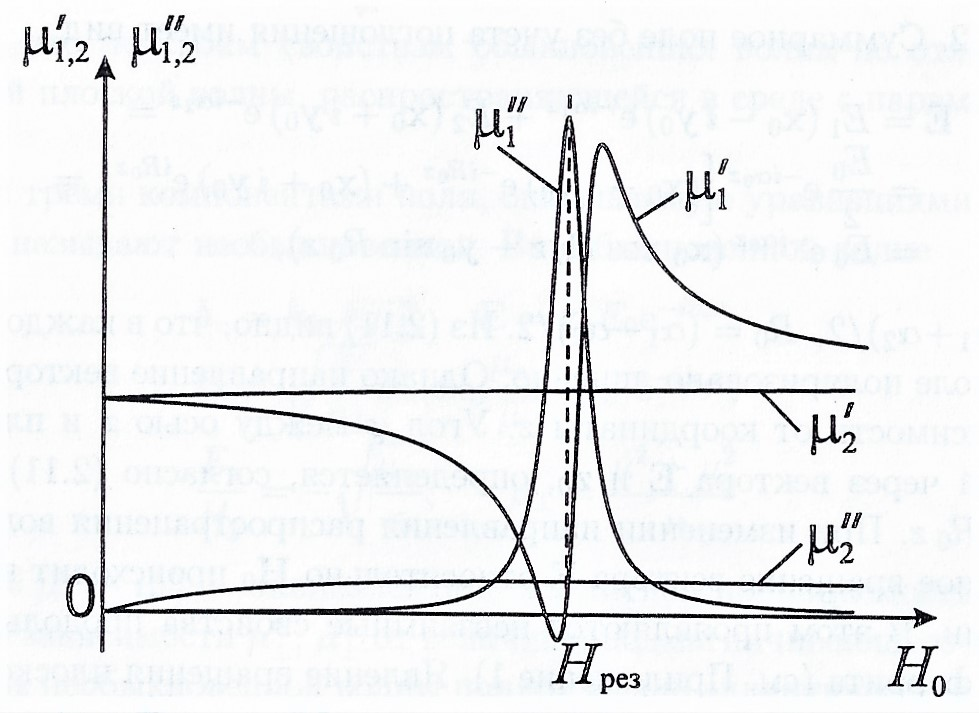
\includegraphics[width = 0.6\linewidth]{imgs/temp/002.JPG}
    \caption{Зависимости действительных и мнимых частей эквивалентных магнитных проницаемости
    $\mu_{1,2}=\mu_{1,2}^{\prime}-i \mu_{1,2}^{\prime \prime}$ для волн с правой и левой круговой поляризацией в
    продольно намагниченном феррите от величины подмагничивающего поля}
    \label{fig:3}
\end{figure}
Нужно подчеркнуть, что направление вращения (правое или левое) для волн с круговой поляризацией определяется
относительно оси $z$, которая всегда совмещается с направлением постоянного поля подмагничивания, независимо от того, в
каком направлении происходит распространение волны. При распространении в отрицательном направлении оси $z$
левополяризованная относительно направления распространения волна обладает теми же свойствами, что и правополяризованная
относительно $\vH_0$ волна, распространяющаяся в сторону положительных значений $z$. Аналогичное утверждение справедливо и в
отношении волны с противоположным направлением вращения векторов $\vE,\vH$.

Рассмотрим распространение в феррите двух волн с левым и правым направлениями вращения векторов ноля и одинаковыми
амплитудами $E_1 = E_2=E_0/2$. Суммарное поле без учета поглощения имеет вид:
\begin{equation}
\begin{aligned} 
    \vE &=E_{1}\left(\vx_{0}-i \vy_{0}\right) e^{-i \alpha_{1} z}+E_{2}\left(\vx_{0}+i \vy_{0}\right) e^{-i \alpha_{2} z}=\\
    &=\frac{E_{0}}{2} e^{-i \alpha_{0} z}\left[\left(\vx_{0}-i \vy_{0}\right) e^{-i R_{0} z}+\left(\vx_{0}+i \vy_{0}\right) e^{i R_{0} z}\right]=\\
    &=E_{0} e^{-i \alpha_{0} z}\left(\vx_{0} \cos R_{0} z-\vy_{0} \sin R_{0} z\right)
 \end{aligned}
    \label{eq:2:11}
\end{equation} 
где $\alpha_{0}=\left(\alpha_{1}+\alpha_{2}\right) / 2, R_{0}=\left(\alpha_{1}-\alpha_{2}\right) / 2$. Из \eqref{eq:2:11} видно,
что в каждом сечении $z = \const$ поле поляризовано линейно. Однако направление вектора $\vE$ меняется в зависимости от
координаты $z$. Угол $\varphi$ между осью $x$ и плоскостью, проходящей через
вектора $\vE$ и $\vz_0$, определяется, согласно \eqref{eq:2:11}, выражением $\varphi=R_{0} z$. При изменении направления распространения волн на
противоположное вращение вектора $\vE$ относительно $\vH_0$ происходит в прежнем направлении. В этом проявляются невзаимные
свойства продольно намагниченного феррита. Явление вращения плоскости поляризации в магнитоактивной
среде называют \textit{эффектом Фарадея}, а величину $R_{0}=k_{0}
\sqrt{\varepsilon}(\sqrt{\mu^{\prime}+\mu_{a}^{\prime}}-\sqrt{\mu^{\prime}-\mu_{a}^{\prime}}) / 2$, определяющую
скорость вращения плоскости поляризации, — \textit{постоянной Фарадея}.
\subsubsection{Поперечное распространение электромагнитных волн в гиромагнитной среде}
Рассмотрим однородную плоскую волну, распространяющуюся в феррите вдоль оси $z$ перпендикулярно направлению подмагничивающего поля $\vH_0=H_0 \vz_0$. 

Волна, распространяющаяся поперек внешнего магнитного поля и имеющая две составляющих поля, называется обыкновенной волной. Она описывается уравнениями:
\begin{equation}
    \begin{array}
    	{ll}{E_0=0,~ hE_y = k_0\mu_{||}H_z,~ hH_z=k_0\varepsilon E_y}, \end{array}
    \label{eq:2:12}
\end{equation}
из которых находим:
\begin{equation}
    \begin{array}
    	{ll}{h_0=k_0\sqrt{\varepsilon \mu_{||}},~\vE=\vy_0 E_0 e^{-ih_0x},~\vH=\vz_0 \sqrt{\frac{\varepsilon}{\mu_{||}}} E_0e^{-ih_0x}, \frac{E_y}{H_z}=\sqrt{\frac{\mu_{||}}{\varepsilon}}}. \end{array}
    \label{eq:2:13}
\end{equation}

Очевидно, по своим свойствам обыкновенная волна не отличается от однородной плоской волны, распространяющейся в среде с параметрами $\varepsilon$ и $\mu=\mu_{||}$.

Волну с тремя компонентами поля, описываемую уравнениями:
\begin{equation}
    \begin{array}
    	{ll}{\mu H_x=-i\mu_a H_y,~ hH_y = -k_0\varepsilon E_z,~ hE_z=-k_0(-i\mu_a H_x + \mu H_y)}, \end{array}
    \label{eq:2:14}
\end{equation}
называют необыкновенной. В ней
\begin{equation}
    \begin{array}
    	{ll}{h_e=k_0\sqrt{\varepsilon \mu_{\bot}},~\vE=\vz_0 E_0 e^{-ih_ex}}, \\ 
    	{\vH= \sqrt{\frac{\varepsilon}{\mu_{\bot}}} E_0(i\vx_0 \frac{\mu_a}{\mu}-\vy_0)e^{-ih_ex}}, \\
    	{\frac{E_z}{H_y}=-\sqrt{\frac{\mu_{\bot}}{\varepsilon}},~\mu_{\bot}=\frac{\mu^2-\mu_a^2}{\mu}}. \end{array}
    \label{eq:2:15}
\end{equation}
Здесь $\mu_{\bot}=\mu_{\bot}^{\prime}-i\mu_{\bot}^{\prime \prime}$ - эквивалентная магнитная проницаемость. На рис. \ref{fig:3} приведены зависимости $\mu_{\bot}^{\prime}$ и $\mu_{\bot}^{\prime \prime}$ от величины подмагничивающего поля. магнитное поле необыкновенной волны поляризовано эллиптически в плоскости $xOy$, перпендикулярной вектору $\vH_0$.
\begin{figure}[H]
    \centering
    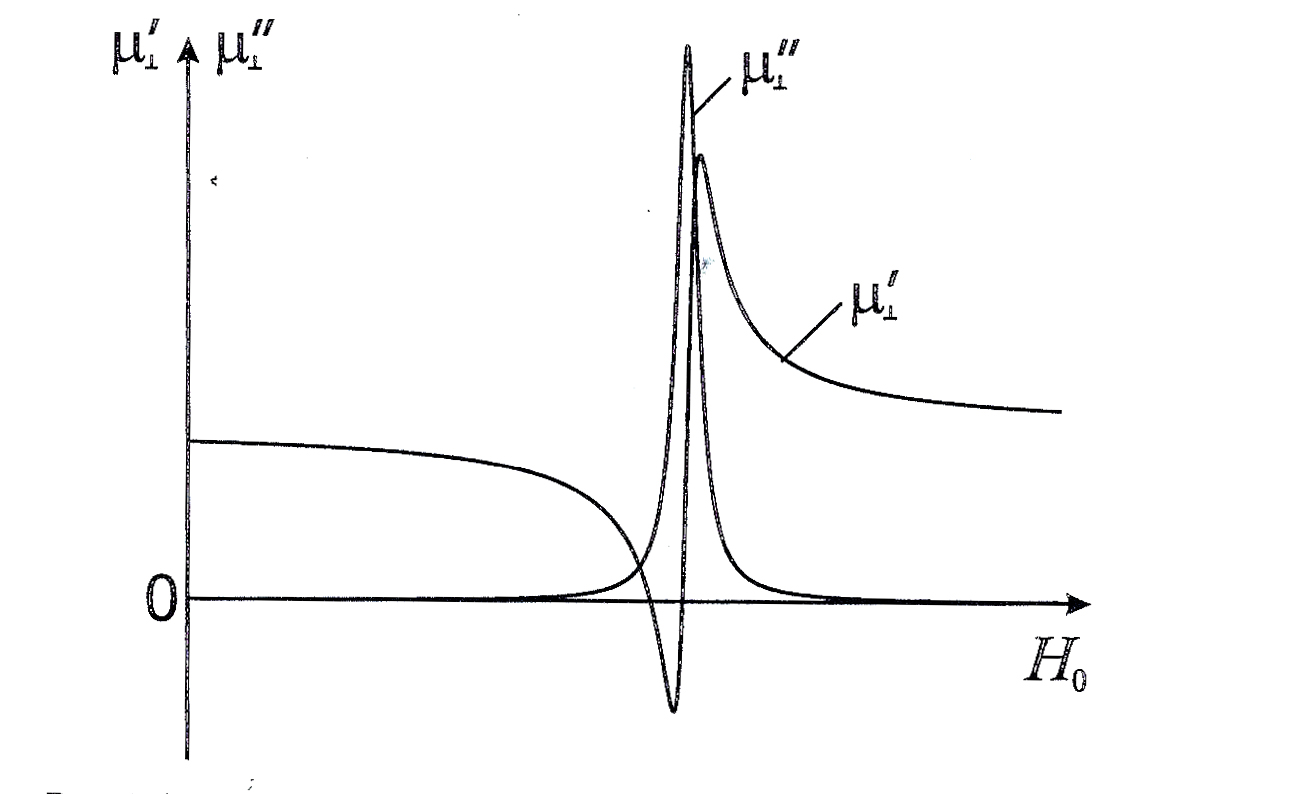
\includegraphics[width = 0.6\linewidth]{imgs/temp/004.JPG}
    \caption{Зависимости действительной и мнимой частей эквивалентной магнитных проницаемости
    $\mu_{\bot}$ для волны, распространяющейся поперек внешнего магнитного поля, от величины этого поля}
    \label{fig:4}
\end{figure}
\subsection{Прямоугольный волновод с продольно намагниченным ферритовым стержнем}
Рассмотрим волновод прямоугольного сечения, в который помещен тонкий продольно намагниченный ферритовый стержень. Будем считать, что частота поля такова, что единственной распространяющейся модой волновода является волна $TE_{10}$. При изменении направления распространения волны, т.е. смене знака постоянной распространения h, величина изменения этой постоянной распространения $\Delta h$ также меняет знак, оставаясь постоянной по абсолютному значению. Следовательно, оба направления распространения равноправны и отрезок прямоугольного волновода с продольно намагниченным ферритом представляет собой взаимное устройство. Такой отрезок волновода может служить для изменения фазы волны с помощью статического магнитного поля.
\subsection{Круглый волновод с продольно намагниченным ферритовым стержнем}
Рассмотрим распространение электромагнитных волн в круглом волноводе, на оси которого размещается тонкий продольно намагниченный ферритовый стержень. Наличие двух собственных функций, отвечающих одной и той же постоянной распространения, означает, что волна $TE_{11}$ круглого волновода является двукратно вырожденной. Наличие ферритового стержня приводит к снятию вырождения между двумя волнами $TE_{11}$ круглого волновода: в одном направлении распространяются две циркулярно поляризованные волны $TE_{11}$ с противоположными направлениями вращения полей и с разными значениями постоянных распространения. Происходит необратимое вращение плоскости поляризации волны, поступающей на вход системы (эффект Фарадея).
\subsection{Прямоугольный волновод с поперечно намагниченной ферритовой пластинкой}
Рассмотрим прямоугольный волновод, содержащий тонкую ферритовую пластинку, намагниченную поперечно по отношению к оси волновода. Если статическое магнитное поле отсутствует, то оба направления распространения волны равноправны. Если статическое магнитное поле отлично от нуля, то постоянные распространения, соответствующие различным направлениям распространения, отличны друг от друга. Поэтому сдвиг фазы волны на отрезке волновода, содержащем поперечно намагниченный феррит, является невзаимным. Величина изменения значения постоянной распространения зависит от положения пластины в волноводе. 

\newpage
\section{Экспериментальная часть}

% Схема установки:
% \begin{figure}[H]
%     \centering
%     \includegraphics[width = 0.7\linewidth]{imgs/exp.png}
% \end{figure}
Оборудование: 
\begin{itemize}
    \item Генератор СВЧ излучения с регулируемыми частотой и ослаблением.
    \item Волноводный переключатель с взаимным фазовращателем
    \item Циркулятор на эффекте Фарадея
    \item Волноводный вентиль
    \item Измерительный тракт
    \item Согласованные нагрузки
\end{itemize}
Во всех экспериментах частота генератора $f_g$ была постоянной и не изменялась: $f_g = 10.6$ ГГц.
\subsection{Волноводный переключатель}
\begin{figure}[h!]
    \centering
    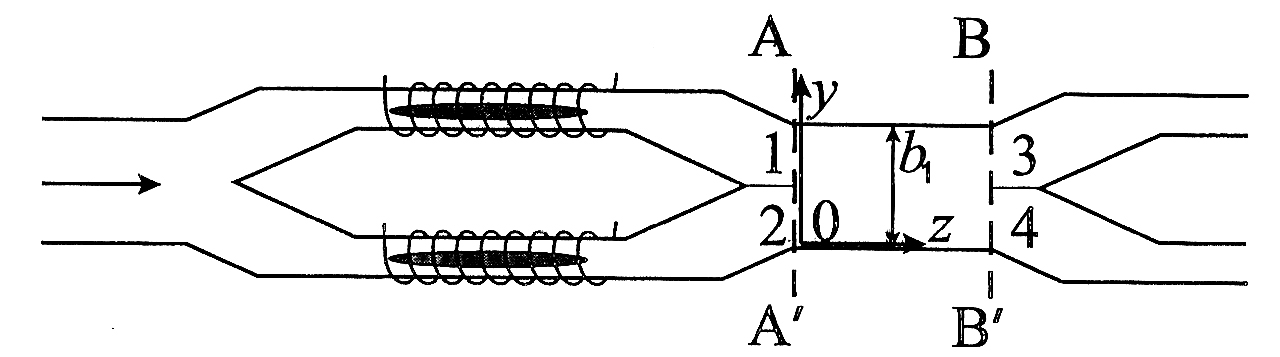
\includegraphics[width = 0.7\linewidth]{imgs/temp/003.jpg}
    \caption{Волноводный переключатель с взаимным фазовращателем}
    \label{fig:ex:1}
\end{figure}
Взаимный фазовращатель представляет собой отрезок прямоугольного волновода с продольно намагниченным ферритом,
расположенным вдоль оси волновода. Путем изменения поля подмагничивания фазовращатель
позволяет регулировать набег фазы на участке волновода с ферритом. Два таких фазовращателя используются в волноводном
переключателе, изображенном схематически на рис. \ref{fig:ex:1}. 
% В переключателе мощность высокочастотных электромагнитных колебаний,
% поступающих из генератора, делится поровну между двумя волноводными секциями, в которых помещены одинаковые ферритовые
% стержни, подмагничиваемые с помощью соленоидов. Размеры секций подобраны таким образом, что в каждой из них (при
% используемой частоте генератора) распространяющейся является только волна низшего типа $TE_{10}$. Затем высокочастотная
% мощность поступает в волноводно-щелевой мост, па выходе которого перераспределяется между двумя волноводами.




% Волноводно-щелевой мост сконструирован таким образом, что мощность, поступающая в любое из его плеч (1 или 2), поровну
% распределяется между противоположными плечами (3 или 4), причем фаза волны в дальнем плече отстает от фазы волны в
% ближнем плече на $\pi/2$. Мост имеет вид сдвоенных прямоугольных волноводов, в общей широкой стенке которых прорезана одна
% или несколько щелей. В лабораторной установке щели прорезаны от одной узкой стенки до другой, а размеры $a_1=a$ и $b_1$
% поперечного сечения области, образованной сдвоенными волноводами (область связи), выбраны такими, чтобы в пей могли
% распространяться волны только трех типов $TE_{10}$, $TE_{01}$, $TE_{11}$.
% \begin{figure}[h!]
%     \centering
%     \includegraphics[width = 0.4\linewidth]{example-image-b}
%     \caption{Векторные диаграммы, поясняющие работу волноводно-щелевого моста}
%     \label{fig:ex:2}
% \end{figure}
% Работу волноводно-щелевого моста удобно пояснить с помощью векторных диаграмм (рис. \ref{fig:ex:2}). На таких диаграммах поле в
% соответствующем плече моста изображается вектором, длина которого равна абсолютному значению поля, а угол поворота
% относительно направления $\phi = 0$ — фазе поля. 

В ходе работы производились измерения мощности на выходе плеч волноводного переключателя, в зависимости от
токов через обмотки фазовращателей. Таблица с измерениями приведена в приложении (см таблицу \ref{tab:phaser}).

Ниже приведены графики зависимости мощности в разных плечах установки от величины тока, протекающего через обмотки фазовращателей.
\begin{figure}[H]
    \centering
    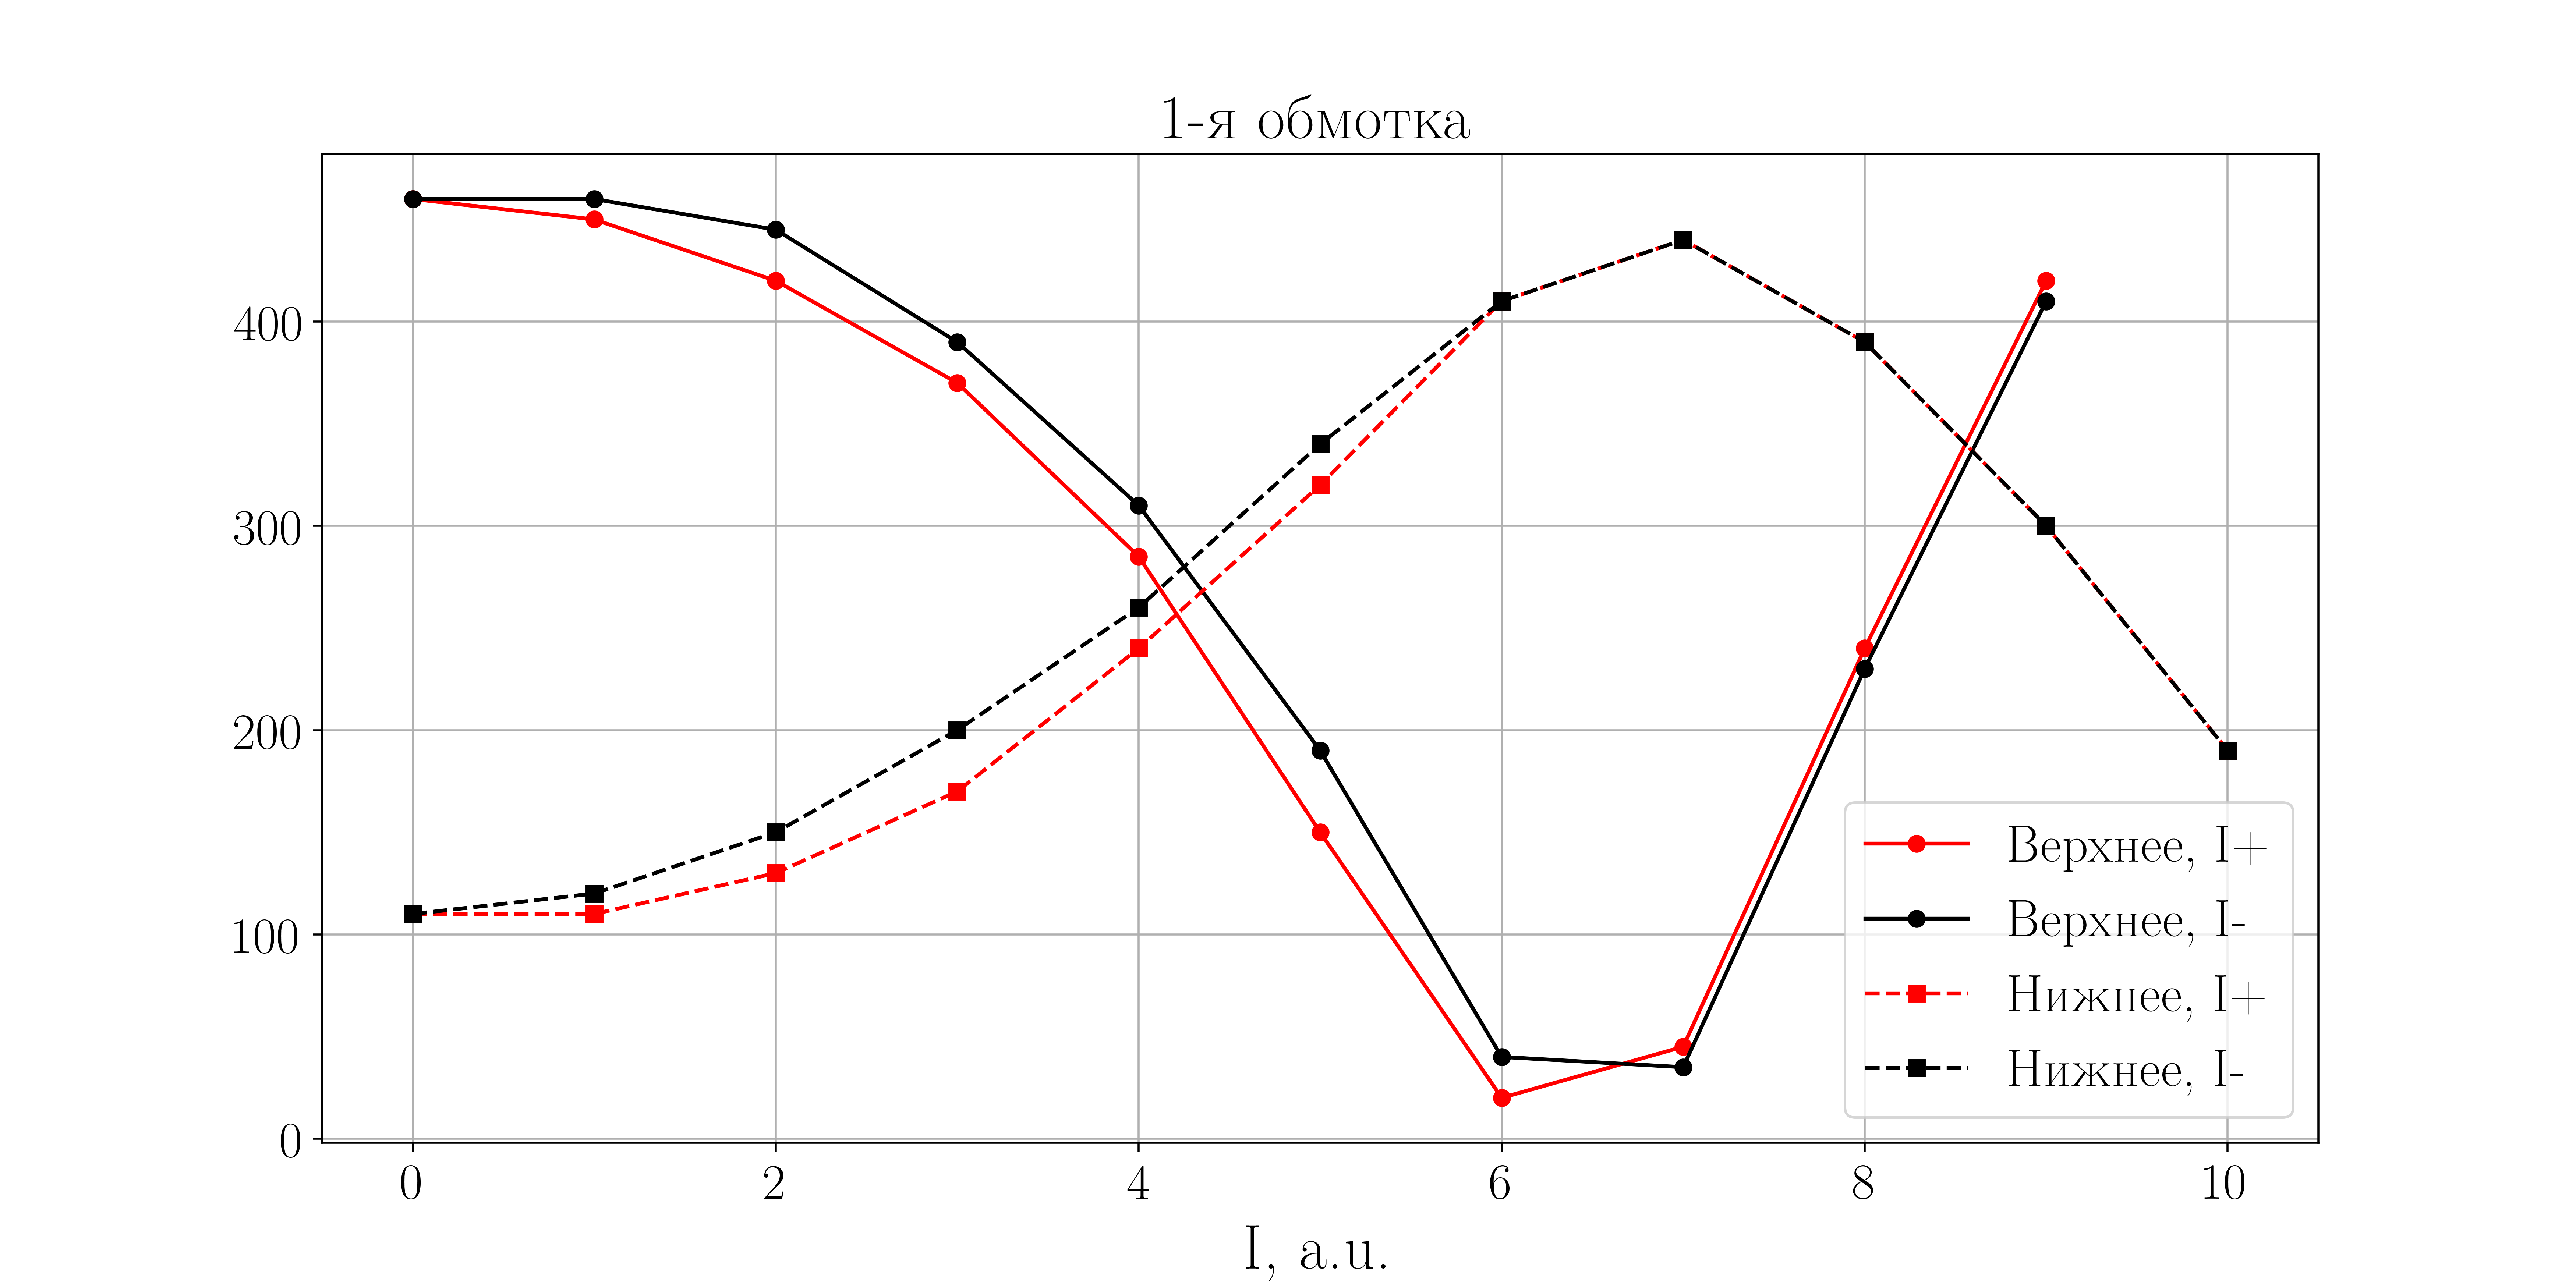
\includegraphics[width = 0.9\linewidth]{imgs/graphs/phaser1.png}
    \caption{Мощность в плечах переключателя от тока в 1й обмотке.}
    \label{fig:exp:phaser1}
\end{figure}
\begin{figure}[H]
    \centering
    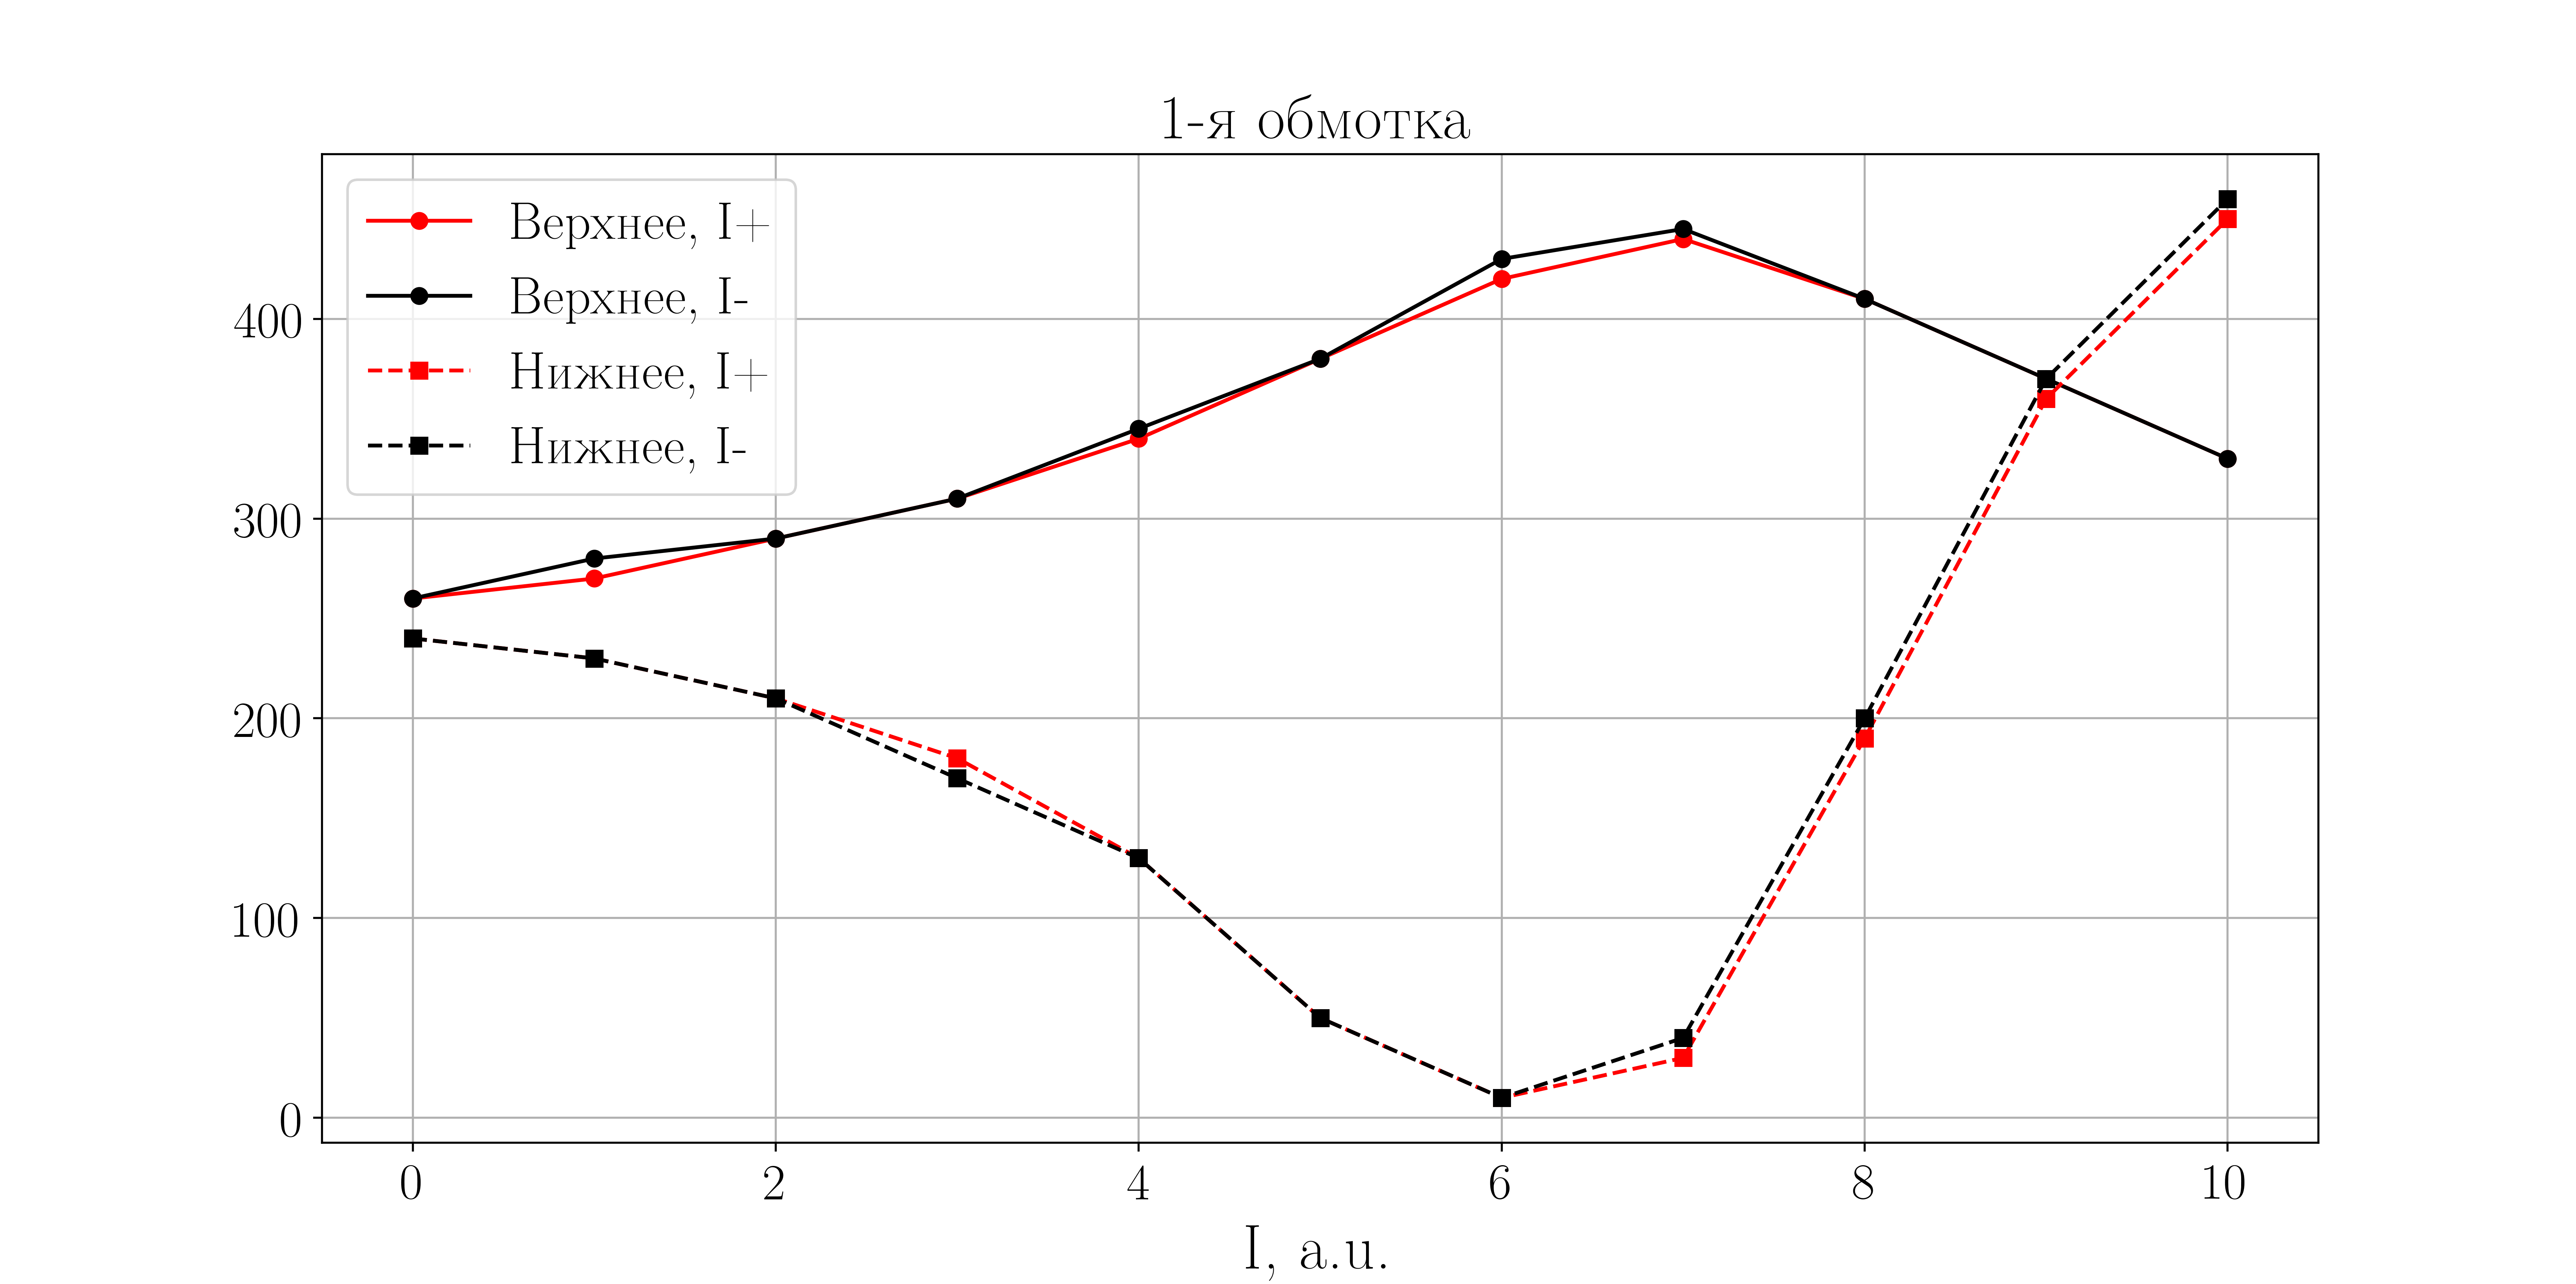
\includegraphics[width = 0.9\linewidth]{imgs/graphs/phaser2.png}
    \caption{Мощность в плечах переключателя от тока во 2й обмотке.}
    \label{fig:exp:phaser2}
\end{figure}
\begin{figure}[H]
    \centering
    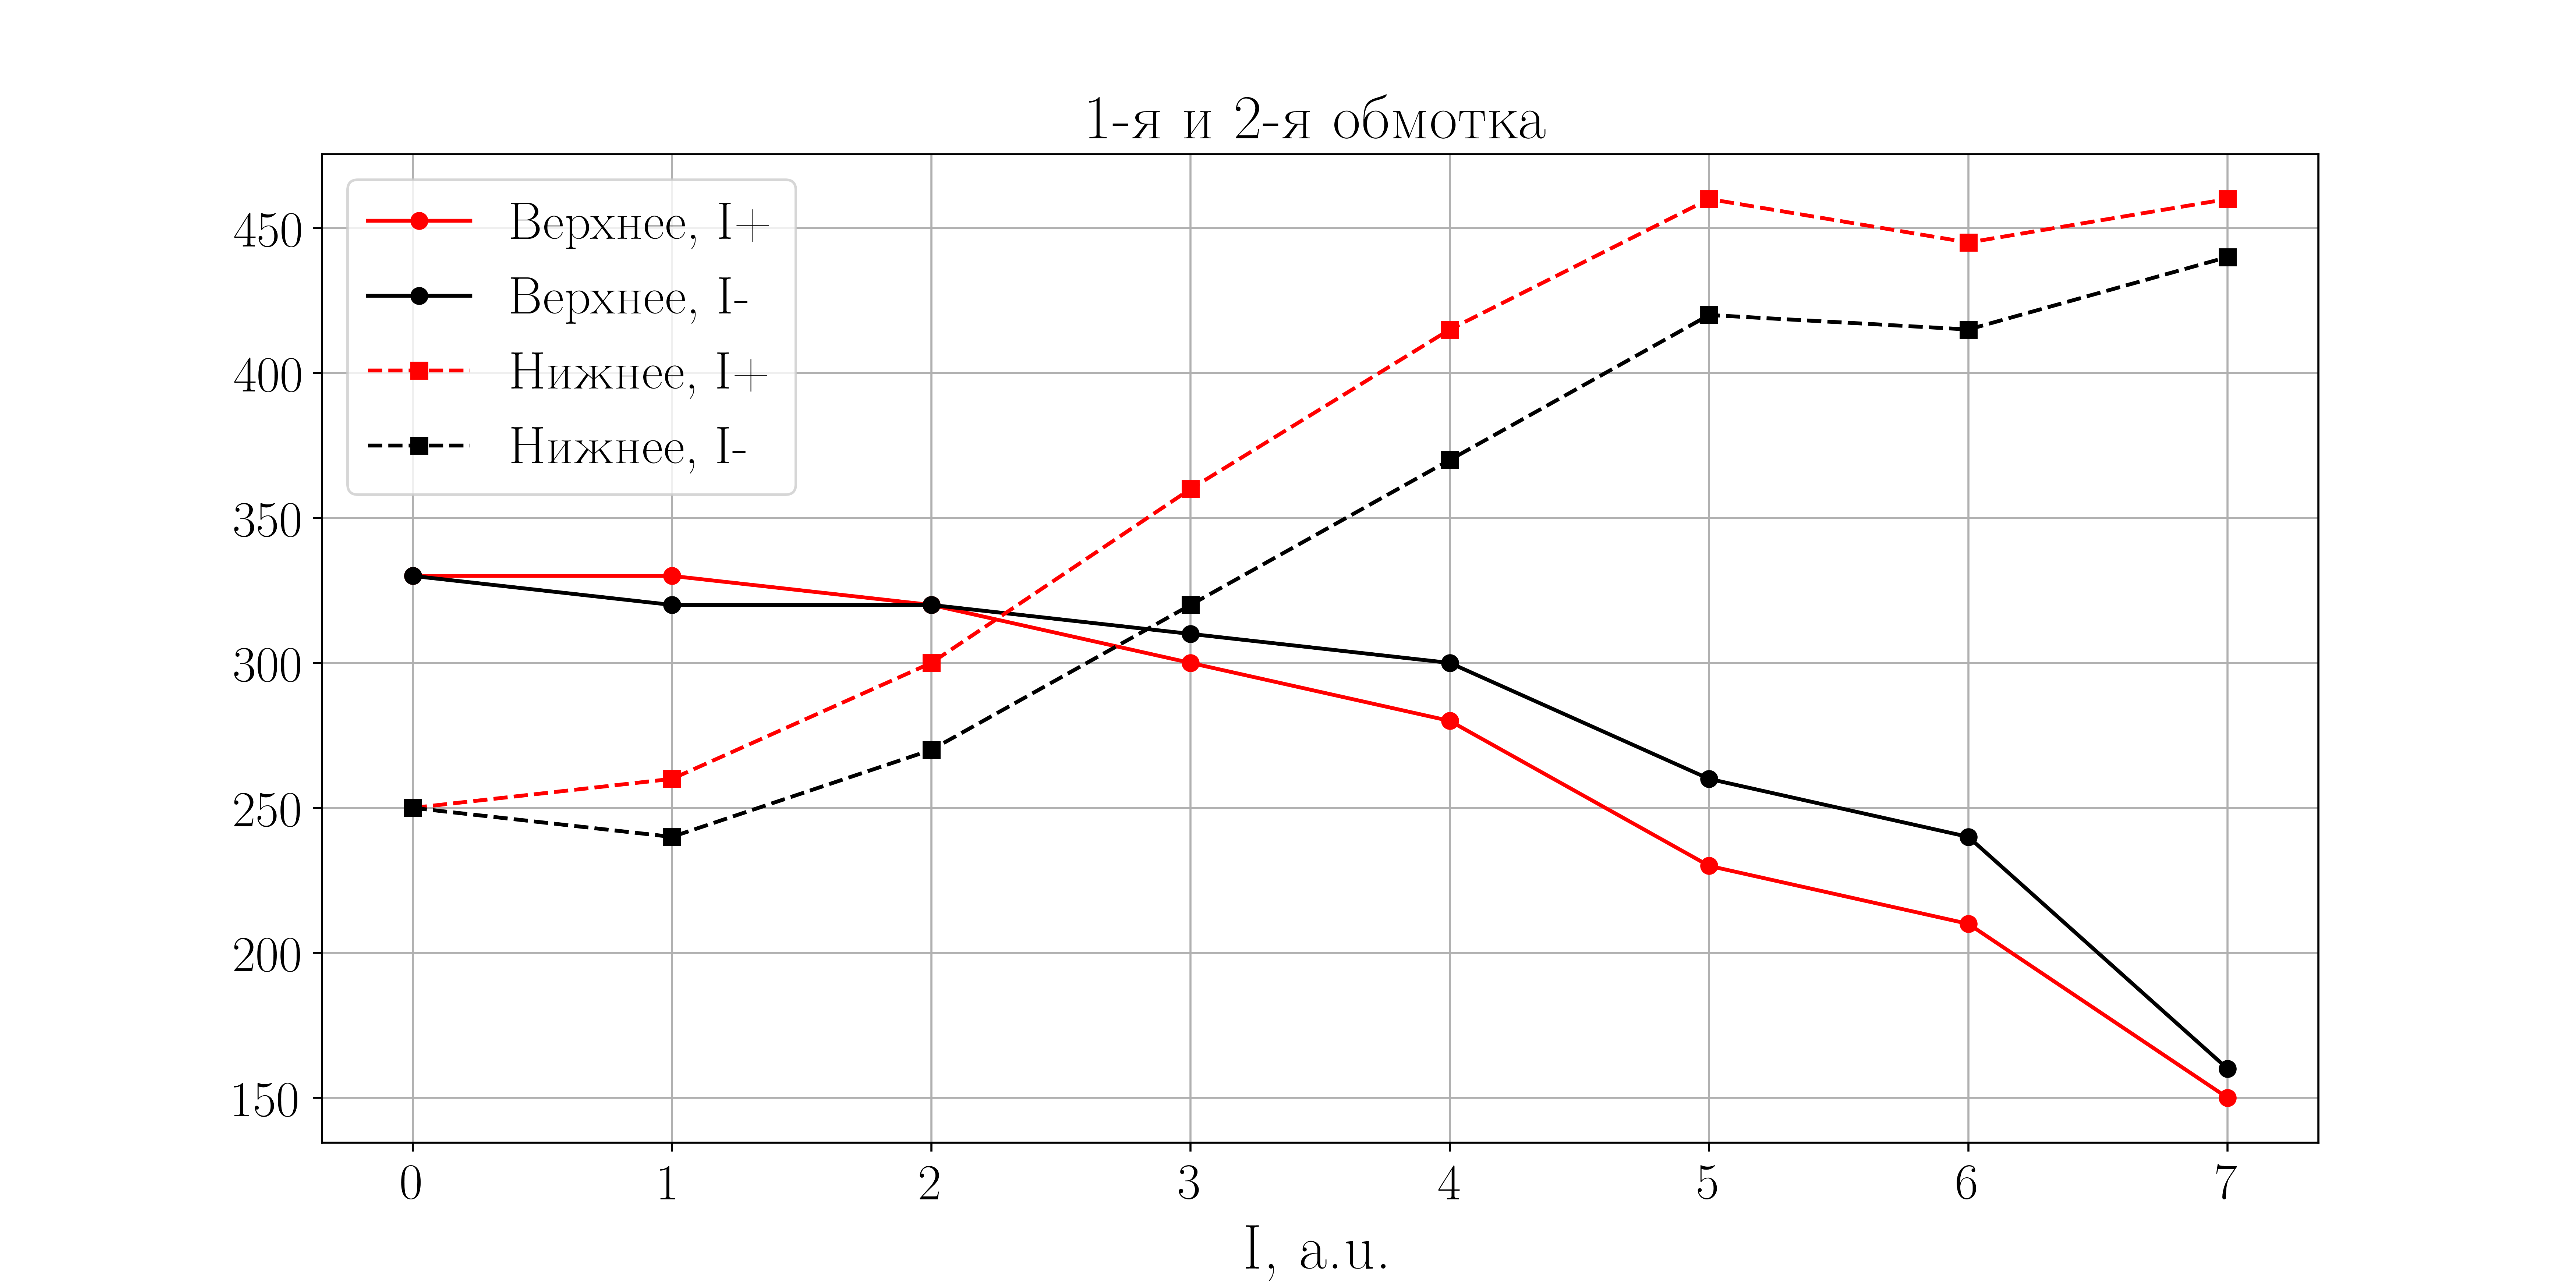
\includegraphics[width = 0.9\linewidth]{imgs/graphs/phaser3.png}
    \caption{Мощность в плечах переключателя от тока в 1й и 2й обмотке.}
    \label{fig:exp:phaser3}
\end{figure}
\subsection{Циркулятор на эффекте Фарадея}
Циркулятор на эффекте Фарадея представляет собой отрезок круглого волновода с помещенным внутри него ферритом,
подмагничивание которого осуществляется продольным полем соленоида. К каждому из концов циркулятора подключены два
взаимно-перпендикулярных волновода, причем волноводы, подходящие к противоположным концам циркулятора, повернуты
относительно друг друга па 45° (рис. \ref{fig:exp:circulator}).
\begin{figure}[h!]
    \centering
    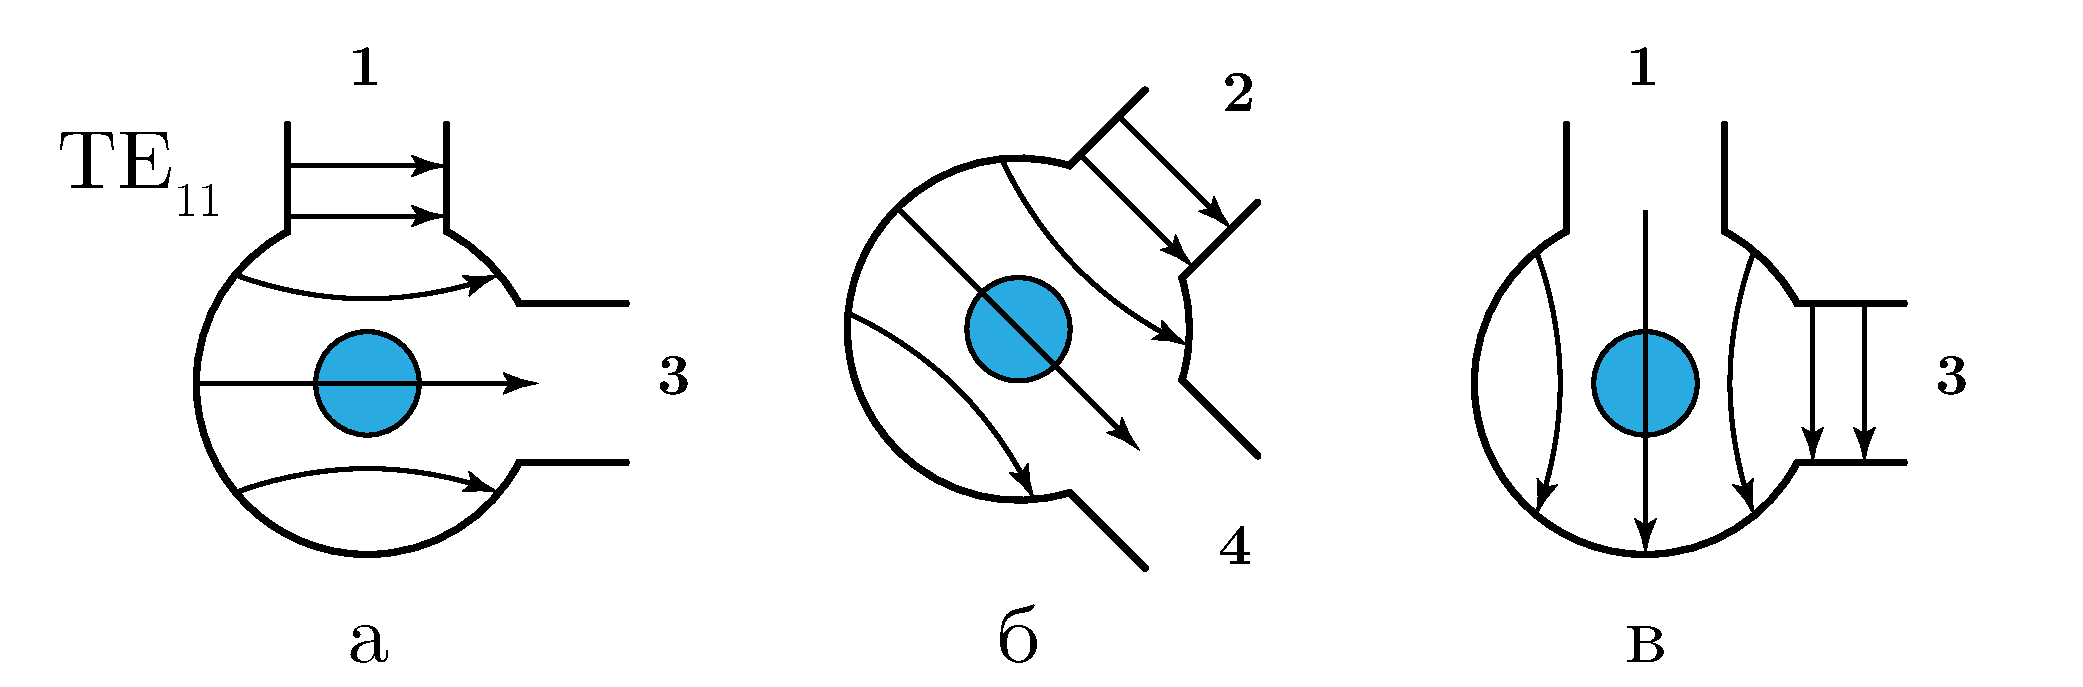
\includegraphics[width = 0.8\linewidth]{imgs/circulator.pdf}
    \caption{Схема работы циркулятора на эффекте Фарадея}
    \label{fig:exp:circulator}
\end{figure}
Циркулятор работает следующим образом. Допустим, что высокочастотная мощность поступает в систему через волновод 1.
%  Это
% поле возбуждает в круглом волноводе волну $TE_{11}$ соответствующей поляризации. В рассматриваемом случае, поток энергии
% в волноводе 3 равен нулю и плечо 3 циркулятора не возбуждается (см. рис. \ref{fig:exp:circulator}а).
 При определенном значении поля
подмагничивания в феррите плоскость поляризации волны в противоположном конце круглого волновода оказывается
повернутой на 45° относительно своего исходного положения (см. рис. \ref{fig:exp:circulator}б). В этом случае мощность
поступает в волновод 2, а волновод 4 не возбуждается, т. е. мощность поступает из первого плеча циркулятора во второе.

Если при той же величине поля подмагничивания циркулятор запитывать из второго плеча, плоскость поляризации волны
$TE_{11}$ будет поворачиваться в том же направлении относительно $\vH_0$ (в изображенном случае — по часовой стрелке).
 Такое поле возбуждает лишь 3-й волновод (рис. \ref{fig:exp:circulator}в).

\textbf{в отчет} 

Исследование схемы работы циркулятора на эффекте Фарадея. Схема установки приведена на рис. \ref{fig:exp:circulator2}.
Циркулятор был настроен таким образом, чтобы при подключении генератора к 1-му плечу, при измерении, мощность во 2-й
плече была максимальной, при минимальных мощностях в 3-м и 4-м плечах.

\begin{figure}[h!]
    \centering
    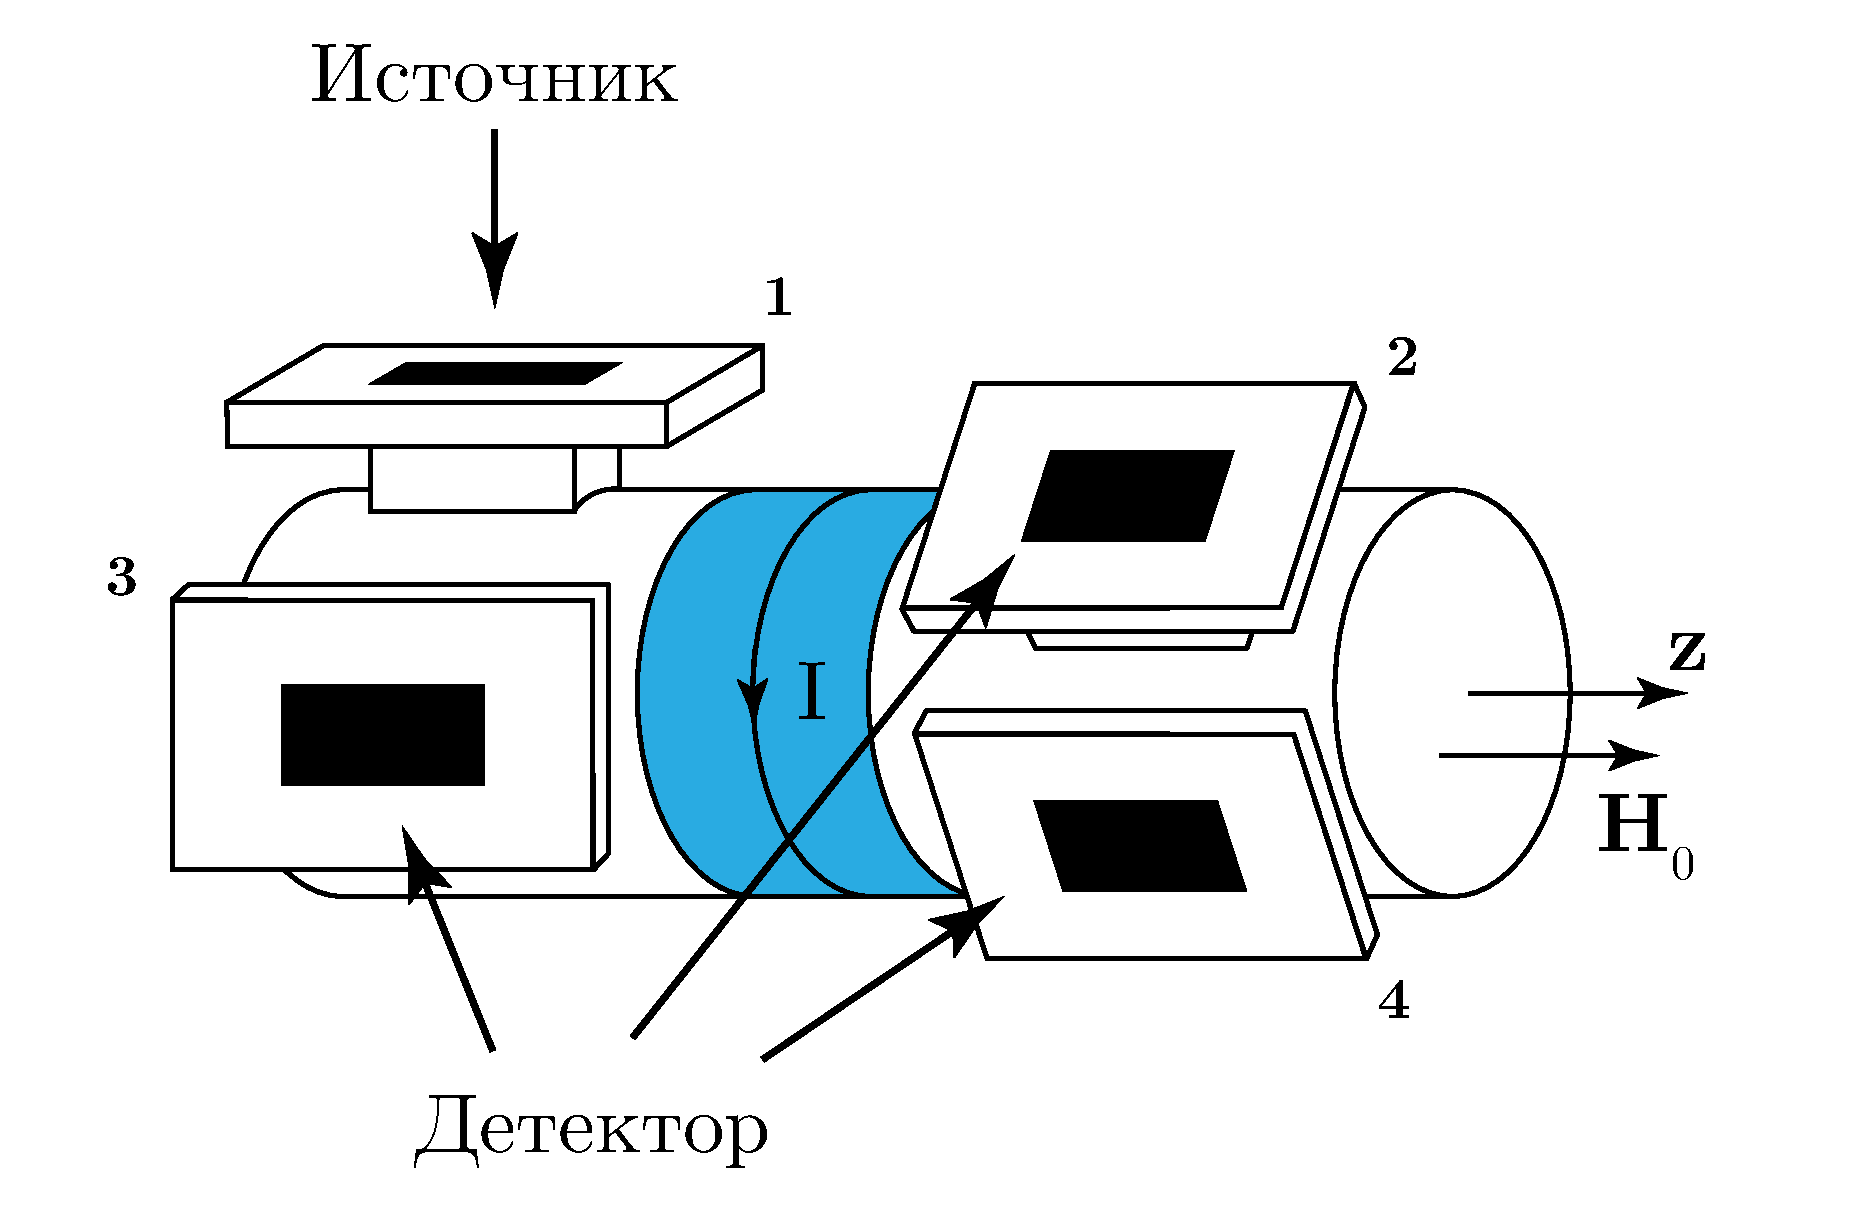
\includegraphics[width = 0.6\linewidth]{imgs/circulator2.pdf}
    \caption{Схема установки с циркулятором}
    \label{fig:exp:circulator2}
\end{figure}

Источник поочередно подключался ко всем 4-м волноводам. Измерения проводились
на оставшихся 3-х волноводах, при этом волноводы замыкались согласованной
нагрузкой. Произведенные замеры приведены в таблице \ref{tab:faradey}.
 \begin{table}[h!]
    \centering
    \begin{tabular}{|c|c|c|c|c|}
    \hline
     $k \textbackslash i$ & 1 & 2 & 3 & 4 \\ \hline
    1 & \cellcolor{black!70}  & $\frac{85}{370}$ & $\frac{0}{0}$& $\frac{360}{40}$  \\ \hline
    2 & $\frac{410}{110}$  &\cellcolor{black!70}   & $\frac{110}{360}$  & $\frac{80}{100}$  \\ \hline
    3 & $\frac{0}{0}$  & $\frac{360}{100}$  & \cellcolor{black!70}  &  $\frac{60}{350}$ \\ \hline
    4 & $\frac{40}{380}$  & $\frac{65}{65}$  & $\frac{360}{70}$  & \cellcolor{black!70} \\ \hline
    \end{tabular}
    \caption{$i$ - номер волновода, к которому подключен источник, $k$ - номер волновода, с которого снимаются
    показания. Верхние значения соответствуют «положительному» направлению тока через обмотку, а нижние - «отрицательному»}
    \label{tab:faradey}
    \end{table}

Исходя из измерений, можно сказать, что циркулятор работает, в соответствии с теорией. Основной процент мощности, при
«положительном» токе, циркулирует следующим образом : $1 \rightarrow 2 \rightarrow 3 \rightarrow 4 \rightarrow 1$, и
в обратном направлении при «отрицательном» токе (т.е. $1 \rightarrow 4 \rightarrow 3 \rightarrow 2 \rightarrow 1$ ).

Так как поворот плоскости поляризации при распространении в положительном направлении оси $z$ происходит по часовой
стрелке (относительно оси $z$ при положительном $R_0$), то в эксперименте, при «положительном» токе, направление оси $z$ совпадает с
направлением на рис. \ref{fig:exp:circulator2}. При «отрицательном» токе, направление напряженности магнитного поля
$\vH_0$ меняется, вместе с направлением оси $z$ (см. рис. \ref{fig:exp:circulator3} ).
\begin{figure}[h!]
    \centering
    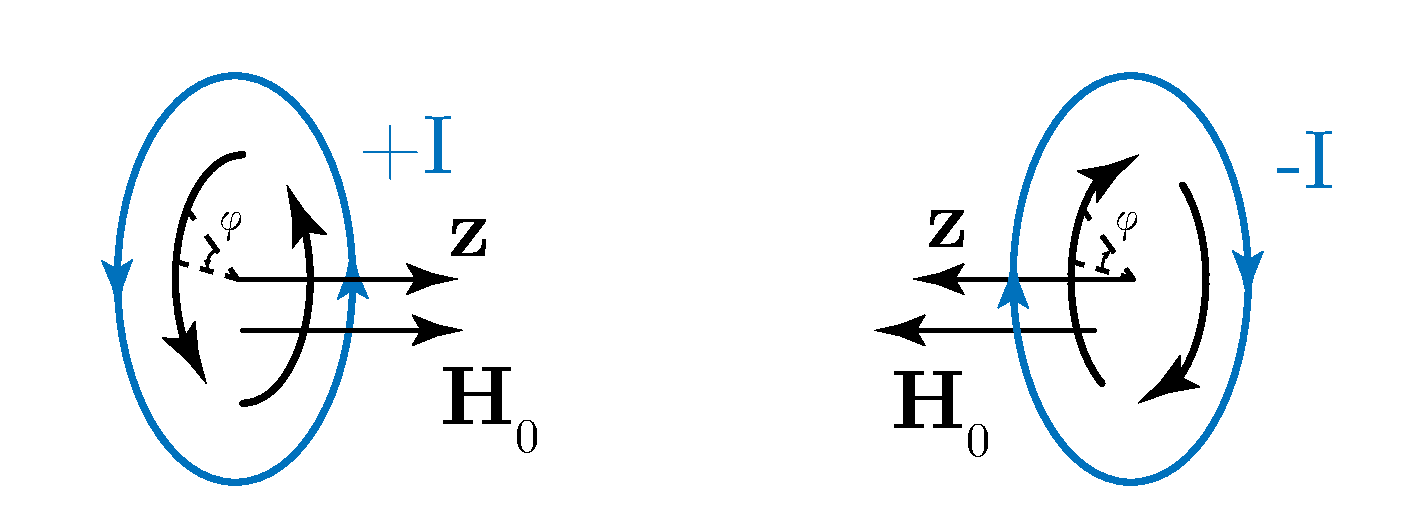
\includegraphics[width = 0.7\linewidth]{imgs/circulator3.pdf}
    \caption{Напрявление протекания тока и поворота плоскости поляризации.}
    \label{fig:exp:circulator3}
\end{figure}
\subsection{Волноводный вентиль}

\subsection{Вывод}

\newpage
\section{Приложение}
\begin{table}[h!]
    \centering
    \begin{tabular}{|c|c|c|c|c|}
    \hline
     $k \textbackslash i$ & 1 & 2 & 3 & 4 \\ \hline
    1 & \cellcolor{black!70}  & $\frac{85}{370}$ & $\frac{0}{0}$& $\frac{360}{40}$  \\ \hline
    2 & $\frac{410}{110}$  &\cellcolor{black!70}   & $\frac{110}{360}$  & $\frac{80}{100}$  \\ \hline
    3 & $\frac{0}{0}$  & $\frac{360}{100}$  & \cellcolor{black!70}  &  $\frac{60}{350}$ \\ \hline
    4 & $\frac{40}{380}$  & $\frac{65}{65}$  & $\frac{360}{70}$  & \cellcolor{black!70} \\ \hline
    \end{tabular}
    \caption{Протокол волноводного переключателя}
    \label{tab:phaser}
    \end{table}


\end{document}